\documentclass[11pt,a4paper]{article}
\usepackage[T1]{fontenc}
\usepackage[utf8]{inputenc}
\usepackage{lmodern}
\usepackage[margin=2.4cm]{geometry}
\usepackage{amsmath,amssymb}
\usepackage{booktabs}
\usepackage{array}
\usepackage{tabularx}
\usepackage{enumitem}
\usepackage{xcolor}
\usepackage[numbers,sort&compress]{natbib}
\usepackage{graphicx}
\usepackage{tikz}
\usetikzlibrary{positioning,arrows.meta,fit,backgrounds,calc,shapes.geometric}
\usepackage[hidelinks]{hyperref}
\definecolor{cM}{HTML}{2457D6}\definecolor{cD}{HTML}{1E8A4C}\definecolor{cP}{HTML}{8A2BD6}
\definecolor{cG}{HTML}{C2620A}\definecolor{cA}{HTML}{C0262D}\definecolor{cE}{HTML}{1F3A5F}
\definecolor{cBg}{HTML}{F3F5FA}\definecolor{cLine}{HTML}{9AA5B8}
\setlist{nosep}\setlist[itemize,enumerate]{leftmargin=*}
\emergencystretch=3em
\newcommand{\code}[1]{\texttt{#1}}

\title{Academic Paper Reviewer: A Multi-Perspective Review Skill\\
for Computer Vision and Machine Learning Papers\\[4pt]
\large Technical Report, version 2.10.1}
\author{Academic Paper Reviewer project\\
\small\url{https://github.com/Shyandram/academic-paper-reviewer.skill}}
\date{November 2026}

\begin{document}
\maketitle

\begin{abstract}
We describe \emph{Academic Paper Reviewer}, a Markdown skill for Claude and Codex agents that
simulates an editorial process for a manuscript. The process has a field-aware panel of five
independent reviewers, a literature check that cannot find the paper under review, a report check,
and an Editor-in-Chief (EIC) who weights each review by its quality and makes the decision.
Scores are aggregated by a deterministic, standard-library Python script and translated into the
forms of 11 venues.

We evaluate the skill in four ways.
\begin{itemize}
\item \textbf{Accepted papers with planted flaws.} On 30 recently accepted CVPR/ECCV/ICLR papers,
96\% of cited locations, 99\% of quoted phrases and all but two of 842 quoted numbers are found in the
paper, and the reviewers mention all six planted fatal flaws.
\item \textbf{ICLR 2026 calibration.} This follows the paperreview.ai protocol. On the balanced
86-paper set with Sonnet at high effort, the reviewers' mean rating reaches Spearman $0.47$
[$0.27$, $0.64$] with the mean human rating (two human reviewers of the same papers: $0.14$) and
an acceptance AUC of $0.64$. On the ICLR scale the normalized mean absolute error is $0.084$,
with essentially no bias (NME $-0.003$). The 20-paper pilot gave the same ranking ($0.48$).
\item \textbf{Weaknesses compared with the human reviews.} On the same 86 papers the panel
raises 46\% of the human reviewers' main issues and 74\% of those two or more reviewers share;
the more important the issue (consensus, a reject vote, a reviewer's lead point), the more often
it is raised. The EIC's five top concerns match human issues more often than an average panel
issue (34\% vs 26\%) but hold only a third of the consensus issues. On a 20-paper pilot, an
optional Gap Scout that names concrete missing items raises 65\% alone and 73\% with the panel.
A redesign that moved these ideas into the panel (version 2.11) raised no more issues, ranked
papers worse (Spearman $0.32$) and cost 3.5$\times$ as much, so it was withdrawn.
\item \textbf{The same model without the skill.} On the same 86 papers, one plain review by the
same model at the same effort agrees with the human reviewers as well as the skill does: Spearman
$0.45$ against $0.47$, AUC $0.63$ against $0.64$, and 46\% against 48\% of the human main issues,
at about a tenth of the cost. Every difference has a 95\% interval that includes zero. On three
papers with 15 planted defects the skill finds all 15 and the plain review 12; the three it misses
are numbers that must be checked across tables.
\end{itemize}
A smaller model (Haiku) shows no reliable signal, and neither do two GPT-6.1 models run on the
same 20 papers. We also report a negative result: NMAE alone
does not measure skill on this pool, because a constant predictor scores $0.089$. The main
remaining weakness is compression: 78\% of papers receive the same final rating.
\end{abstract}

\section{Introduction}
Large language models can now write fluent paper reviews. Fluency, however, is not the goal of a
review. Authors need the decisive weaknesses found, grounded in the manuscript, and ranked by how
much they matter at a target venue. Three failure modes are common:
\begin{itemize}
\item \textbf{Ungrounded criticism:} weaknesses that the paper already answers, or locations and
numbers that do not exist.
\item \textbf{Compressed scores:} every paper rated ``borderline''.
\item \textbf{Leakage:} the reviewer finds the paper's own camera-ready version, reviews or
acceptance status, through retrieval or memory.
\end{itemize}

Prior AI reviewers either prompt a general model once per paper, as in the AI
Scientist~\citep{lu2024aiscientist}, or fine-tune an open model on public reviews:
OpenReviewer~\citep{idahl2025openreviewer}, SEA-E~\citep{yu2024sea},
CycleReviewer~\citep{weng2025cycleresearcher} and DeepReviewer~\citep{zhu2025deepreview}.
Academic Paper Reviewer instead addresses these failure modes with structure rather than with a
single prompt or a single trained model.
\begin{itemize}
\item Several reviewers with distinct roles write independently.
\item A Devil's Advocate attacks the paper.
\item A report check removes ungrounded points.
\item An EIC acts as area chair.
\end{itemize}
The skill is tuned for computer vision, deep learning and ML papers, with task-specific checklists
for detection, segmentation, 3D/NeRF/3DGS, restoration, generation, VLMs, video, medical imaging
and efficient models, but it can be used in any field. Its output is a \emph{simulation} to help
authors improve a paper, not a prediction of a venue's decision.

\paragraph{Contributions.}
\begin{enumerate}
\item A review workflow with independent role-based reviewers, a quality-weighted EIC, and
deterministic score aggregation into venue-specific forms (Section~\ref{sec:system}).
\item Safeguards against prompt injection and self-leakage in literature search
(Section~\ref{sec:safety}).
\item A reproducible calibration harness following the paperreview.ai protocol~\citep{paperreview},
extended with CSPaper-style error metrics~\citep{cspaper} and a no-split pilot mode
(Section~\ref{sec:iclr}).
\item An evaluation on 86 ICLR 2026 papers of both the ratings (Section~\ref{sec:iclr}) and the
stated weaknesses against the human reviews, including whether the important issues and the
EIC's priorities match the humans' (Section~\ref{sec:overlap}); and the pilots that led there,
including what did not work.
\end{enumerate}

\section{System design}\label{sec:system}

\subsection{Workflow}

\begin{figure}[t]
\centering
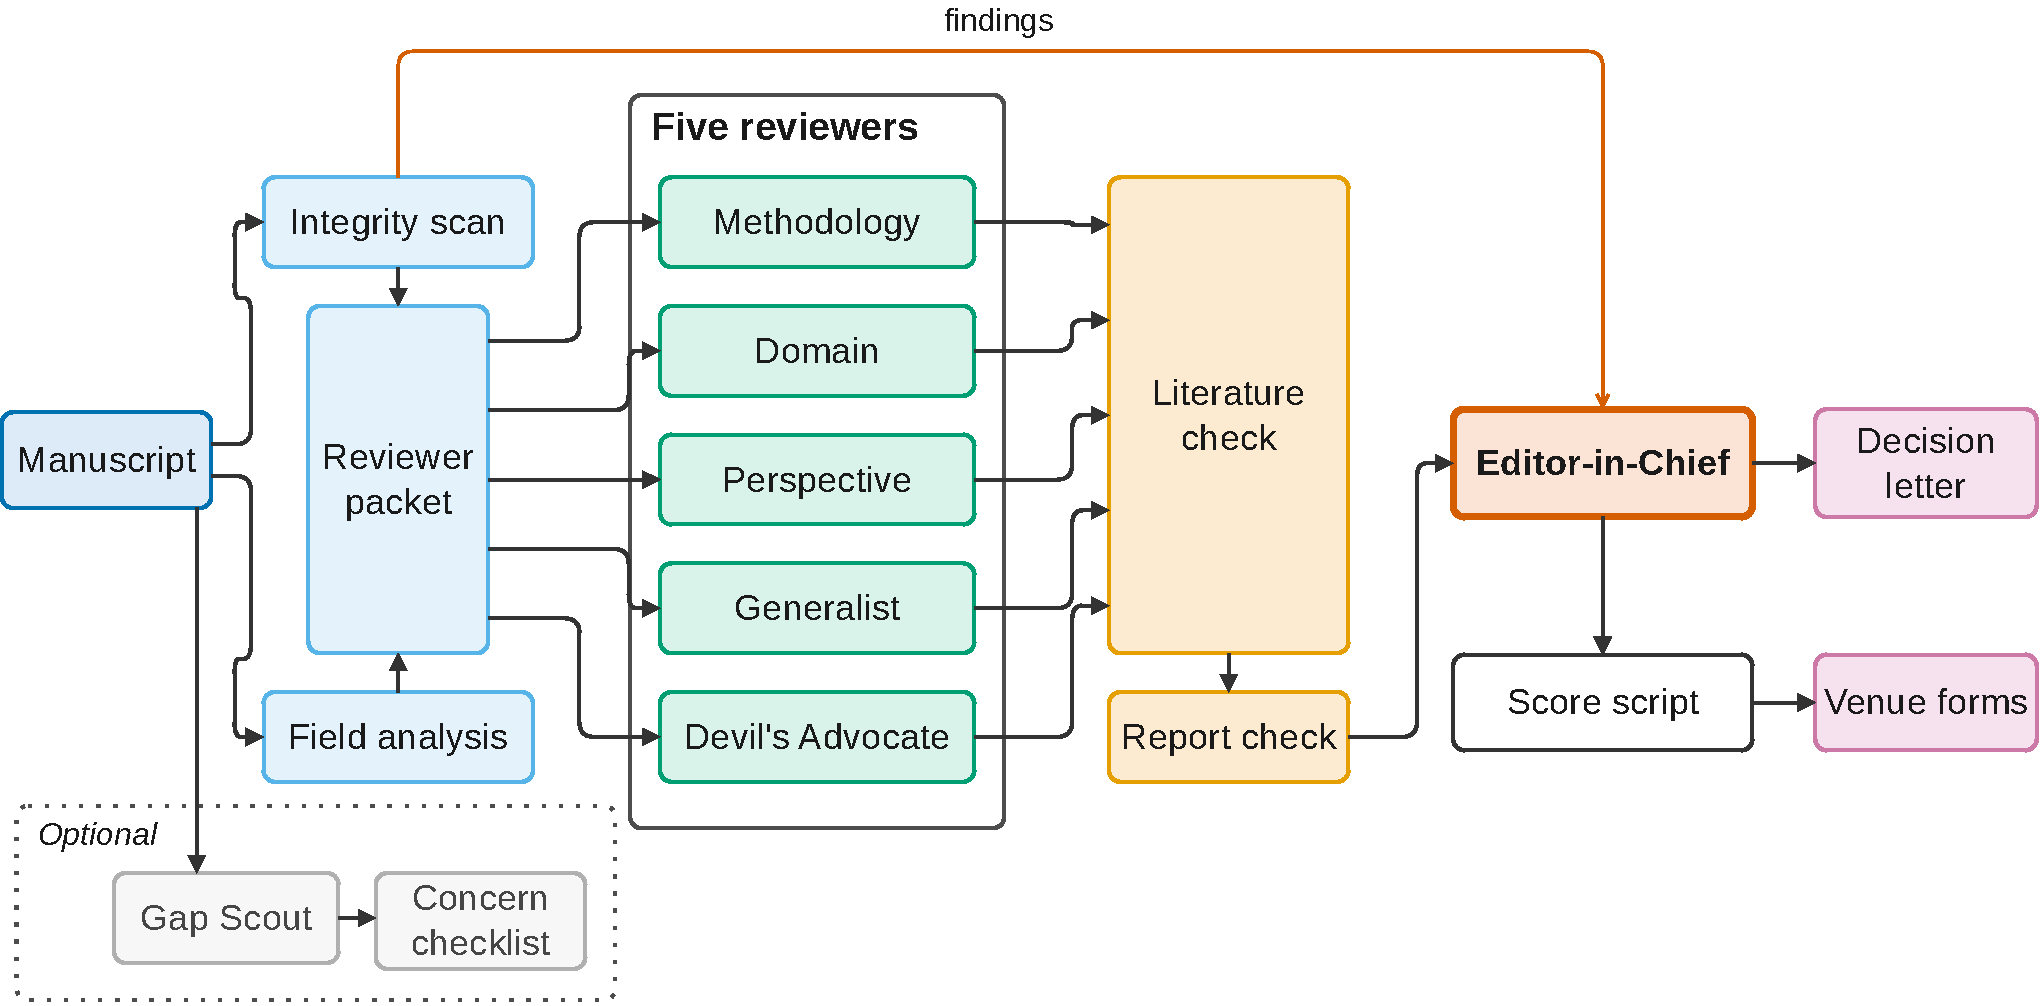
\includegraphics[width=\linewidth]{fig/workflow.pdf}
\caption{Full-mode workflow. Phase~0 analyses the field and configures the panel, and an
integrity scan redacts text addressed to AI reviewers; each reviewer gets the configuration, a
factual paper memory and the redacted copy, never another reviewer's report. The literature check
(Phase~1.5, skipped without network access) cannot retrieve the paper under review; the report check
(Phase~1.6) follows it. The Editor-in-Chief (Phase~2) alone sees the integrity findings (thin
arrow), weights each review by quality and decides; a deterministic script translates the scores
into the forms of 11 venues. The Gap Scout is optional, runs after the review and changes none of
it. Drawn with the paper-figure skill (Draw.io, editable source in \code{report/fig/}).}
\label{fig:workflow}
\end{figure}
A full review runs the phases in Figure~\ref{fig:workflow}. The phases are Markdown instructions in
\code{SKILL.md} and \code{agents/*.md}; scripts are optional helpers.
\begin{description}
\item[Phase 0: field analysis.] A field analyst identifies the paper's sub-field, technique, paper
type (empirical, theoretical, dataset, system, benchmark, analysis, position) and target venue,
and configures five reviewers with specific expertise. An example is ``token pruning + latency
benchmarking'' rather than ``deep learning''. \code{integrity\_scan.py} flags text addressed to
reviewers or AI systems, as well as hidden characters.
\item[Phase 1: independent reviews.] Five reports are written independently: Methodology (R1),
Domain (R2), Perspective (R3), Generalist (R4) and a Devil's Advocate (DA). In Claude Code they can
run as parallel subagents. The Methodology reviewer runs an error audit in nine categories (result
inconsistencies, equation and proof errors, assumptions, protocol flaws, claim distortion,
inconsistent definitions, citation errors, omissions, figure/table integrity). It works from a
shared factual \emph{paper memory}, and every error needs a location, a verbatim quote and a
concrete check.
\item[Phase 1.5: literature check.] This runs only with network access and after the reports are
drafted. Searches are driven by contribution claims and benchmarks: a novelty verdict per claim, a
baseline scout, a coverage pass, a field snapshot and a similarity ranking. Section~\ref{sec:safety}
describes how the paper itself is excluded.
\item[Phase 1.6: report check.] Before the EIC reads anything, vague weaknesses, points the paper
already answers, and claims the paper contradicts are removed. Cosmetic issues are grouped as Minor.
\item[Phase 2: EIC meta-review.] The EIC reads every report and checks the decisive points against
the paper. It assigns each reviewer a quality weight in $[0.5, 1.5]$, states its own pool position,
and decides. Each DA-CRITICAL issue gets an area-chair test (``would I reject on this alone?'').
\end{description}
Other modes reuse the same components: quick assessment, methodology focus, guided (Socratic)
review, rebuttal drafting and re-review of a revision.

\paragraph{Post-review analysis (optional).} After the review, or on its own, the user can ask
for a \emph{Gap Scout}: a separate agent that reads only the redacted paper and lists 20--30
concrete concerns reviewers are likely to raise (the specific missing experiment, baseline,
definition or setting, with a location). It gives no scores, is never called by default and never
changes the review; its list is a checklist for the authors (Section~\ref{sec:overlap}).

\subsection{Scores}
Every non-DA reviewer gives NeurIPS-style 1--4 ratings, an Overall 1--6 recommendation (6 Strong
Accept \dots\ 1 Strong Reject), a confidence 1--5, and seven 0--100 dimension scores: technical
rigor, clarity, novelty, significance, experimental validation, reproducibility and ethics. The DA
gives the 0--100 set only. Dimensions are combined with paper-type weights
(Table~\ref{tab:weights}).

\begin{table}[t]
\centering\small
\caption{Paper-type weights of the seven 0--100 dimensions (each row sums to 1).}
\label{tab:weights}
\begin{tabular}{lccccccc}
\toprule
Type & Rigor & Clarity & Novelty & Signif. & Exp. val. & Repro. & Ethics\\
\midrule
empirical   & .20 & .10 & .15 & .15 & .20 & .10 & .10\\
theoretical & .30 & .10 & .20 & .15 & .10 & .05 & .10\\
dataset     & .15 & .10 & .10 & .20 & .15 & .15 & .15\\
system      & .20 & .10 & .10 & .20 & .20 & .10 & .10\\
benchmark   & .15 & .15 & .10 & .20 & .20 & .15 & .05\\
analysis    & .25 & .10 & .20 & .20 & .15 & .05 & .05\\
position    & .15 & .20 & .25 & .25 & .05 & .00 & .10\\
\bottomrule
\end{tabular}
\end{table}

Two score lists are kept. The \textbf{official} list holds the reviewers' raw ratings and their
plain means, which is what authors see; it is never modified. The \textbf{EIC assessment} weights
reviewer $i$ by
\begin{equation}
w_i = c(\text{conf}_i)\cdot q_i,\qquad c(5..1) = (1.00, 0.85, 0.70, 0.55, 0.40),\quad q_i\in[0.5,1.5],
\end{equation}
where $q_i$ is the EIC's quality weight. The decision starts from the EIC-weighted mean of the
Overall ratings, rounded half up. The weighted 0--100 composite is a cross-check: it maps to
Overall at thresholds 85/70/60/50/35. Two further rules apply:
\begin{itemize}
\item \textbf{DA cap.} Upheld DA-CRITICAL issues cap the decision at 4 if they can be resolved by
clarification and at 3 otherwise.
\item \textbf{Consistency warnings} flag disagreements that the EIC must explain.
\end{itemize}

\paragraph{Calibration to the submission pool (2.10).}
Each reviewer and the EIC first state a \emph{pool position} $P$: the share of the venue's
submissions the paper is better than, using real base rates (about 25\% acceptance at major ML/CV
conferences; ICLR 2026 about 27\% accepted, 45\% rejected, 24\% withdrawn, 5\% desk rejected). They
then score within the matching band:
\begin{center}\small
\begin{tabular}{lcccccc}
\toprule
$P$ & $\ge 95$ & 85--94 & 70--84 & 55--69 & 30--54 & $<30$\\
composite & 85+ & 73--84 & 62--72 & 55--61 & 42--54 & $<42$\\
\bottomrule
\end{tabular}
\end{center}
A composite of 62 is the accept-side bar. Uncertainty is never a reason to score a paper as
borderline. The aggregation script warns when a composite lies more than 5 points outside its
pool band, and when all reviewers sit in the borderline band.

\subsection{Venue forms}
Internal scores are translated into 11 venue forms: CVPR, ICCV, ECCV, NeurIPS, ICLR, ICML,
AAAI, ACM MM, TMLR, IEEE TPAMI and IEEE TIP. Each translation applies the venue's emphasis
weights, bar offset and scale. Each scale is labeled \emph{official}, \emph{confirmed},
\emph{secondary}, \emph{assumed} or \emph{unpublished}. For ICLR 2026 the Overall maps to the
rating set $\{0,2,4,6,8,10\}$ as $r = 2(x-1)$. The legacy (2025) set is $\{1,3,5,6,8,10\}$.

\section{Safeguards}\label{sec:safety}
\begin{itemize}
\item \textbf{Prompt injection.} The manuscript is treated as data, never as instructions.
Injected text is reported to the editor as an integrity concern and never raises a score.
\item \textbf{Self-leak in literature search.} A fingerprint filter refuses queries that could
find the reviewed paper. It drops the paper's own arXiv versions, code pages, reviews and
acceptance lists unread, and labels every other result as prior (peer-reviewed or 6+ months old),
recent preprint, concurrent or newer. Only prior work can be a required comparison. Each run logs
the mode (\code{on}, \code{strict} or \code{off}). In \code{strict} mode a cutoff date applies; in
evaluation this is the submission deadline.
\item \textbf{Recognition.} Reviewers report when they recognize a paper from prior knowledge, and
such papers are reported separately.
\item \textbf{Integrity.} Reviewer personas are fictional, no citations may be fabricated, and
every point is tied to a location in the manuscript.
\end{itemize}

\section{Evaluation I: accepted papers and planted flaws}\label{sec:accepted}
An earlier release of the skill (before 2.10) reviewed 30 recently accepted papers: 10 each from
CVPR, ECCV and ICLR, spread over 10 topics. All runs completed with every required section; the
median review length was 10{,}214 words. Table~\ref{tab:grounding} reports grounding.

\begin{table}[t]
\centering\small
\caption{Grounding on 30 accepted papers: share of cited items not found in the paper.
Numbers the reviewers recomputed themselves (525) are excluded and were spot-checked by hand.}
\label{tab:grounding}
\begin{tabular}{lrrr}
\toprule
Check & Checked & Not found & Rate\\
\midrule
Cited locations (tables, figures, sections, equations) & 1101 & 48 & 4\%\\
Quoted phrases & 778 & 9 & 1\%\\
Quoted numbers & 842 & 2 & 0\%\\
\bottomrule
\end{tabular}
\end{table}

\paragraph{Planted flaws.} In six accepted papers we inserted one sentence admitting a fatal
evaluation flaw: hyperparameters tuned on the test set, or the test split merged into training.
\begin{itemize}
\item The reviews mentioned the flaw in 6/6 papers.
\item The Devil's Advocate raised it as DA-CRITICAL in 2/6, and the EIC upheld both.
\item The final decision was $\le 3$ in 5/6.
\end{itemize}
The miss was an ICLR paper rated 4.

\paragraph{Decisions.} 16/30 accepted papers landed on the accept side (Overall $\ge 4$); 14
received 3. This compression motivated the pool-position calibration of version 2.10. The DA raised
CRITICAL issues on 11/30 papers, and the EIC upheld none on real papers.

\section{Evaluation II: ICLR 2026 ratings}\label{sec:iclr}

\subsection{Protocol}
We follow the paperreview.ai protocol~\citep{paperreview}.
\begin{itemize}
\item Sample ICLR 2026 submissions with human reviews, including withdrawn ones.
\item Fit an ordinary least-squares map from the seven dimension scores to the human rating on a
train split.
\item Report on the test split: Spearman with one human rating, and the AUC of the score for
acceptance. Confidence intervals come from bootstrap resampling; results are given for all scored
papers and without withdrawn papers.
\end{itemize}
The harness (\code{evals/iclr\_calibration.py}, standard library only) runs in GitHub Actions
through the API. Reviewers never see human scores or decisions.

\paragraph{Error metrics.} Following the CSPaper benchmark~\citep{cspaper}, for predictions $\hat s_j$ and human
ratings $s_j$ on a scale $[S_{\min}, S_{\max}]$ (ICLR 2026: $[0,10]$),
\begin{equation}
\mathrm{NMAE} = \frac{1}{n}\sum_{j}\frac{|s_j - \hat s_j|}{S_{\max}-S_{\min}},\qquad
\mathrm{NME} = \frac{1}{n}\sum_{j}\frac{\hat s_j - s_j}{S_{\max}-S_{\min}}.
\end{equation}
We report each with its per-paper standard deviation and a bootstrap 95\% CI. Pilots are too small
to fit the regression, so the \code{pilot} command scores the skill's own outputs as they are,
without any fitting to human scores:
\begin{itemize}
\item the \emph{panel rating}: the reviewers' mean Overall, mapped to the ICLR scale by $2(x-1)$;
\item the \emph{final rating}: the integer decision on the ICLR scale.
\end{itemize}

\subsection{Data and a decision leak}
The sample is ICLR 2026 with seed 2025: 300 papers drawn, 295 with human scores. Our first pilot
used the PDFs from paperreview.ai's dump. These turned out to leak the decision: every accepted
paper was a camera-ready version (author names, acknowledgments, no line numbers), while all other
papers were anonymous submissions. Overall, 0/29 accepted papers and 56/56 other papers showed
``Anonymous authors''. We therefore use only arXiv versions posted before the 2026-01-26 decision
date, normalized identically. The header before the abstract is replaced by the title, and line
numbers, arXiv stamps, emails, affiliation footnotes, code links, acknowledgments and acceptance
marks are removed. The literature check runs in \code{strict} mode with the submission deadline as
cutoff.

The protocol's balanced set has 86 papers (23 accepted, 43 rejected, 17 withdrawn, 3 desk
rejected; 45 train, 41 test). The pilots used 20 of them, stratified by decision and human score:
5 accepted, 10 rejected, 4 withdrawn and 1 desk rejected.

\subsection{Main result: 86 papers}\label{sec:full}
On the balanced set we reviewed the 66 papers not in the pilot with skill 2.10.1,
which keeps the 2.10 panel, scoring and decision, and reused the 20 pilot~3 runs. All 86 runs
finished, at \$166.61 in total (\$1.94 per paper). Table~\ref{tab:full} gives the results.

\begin{table}[t]
\centering\small
\caption{Full evaluation (Sonnet, high effort, 86 papers): the panel rating against the mean
human rating, Spearman [bootstrap 95\% CI] / acceptance AUC, and errors on the ICLR scale.}
\label{tab:full}
\setlength{\tabcolsep}{4pt}\footnotesize
\begin{tabular}{lccc}
\toprule
Papers & $n$ & Spearman & AUC\\
\midrule
All & 86 & $\mathbf{+0.47}$ [$0.27$, $0.64$] & 0.64\\
Pilot 3's papers & 20 & $+0.48$ [$0.10$, $0.74$] & 0.67\\
The 66 new papers & 66 & $+0.48$ [$0.25$, $0.66$] & 0.64\\
Not recognized by the reviewer & 75 & $+0.48$ [$0.28$, $0.65$] & 0.66\\
Without withdrawn papers & 69 & $+0.40$ [$0.17$, $0.59$] & 0.61\\
Test split, against one human (protocol) & 41 & $+0.45$ [$0.14$, $0.69$] & 0.67\\
Protocol regression on 7 dimensions, test split & 41 & $+0.19$ [$-0.13$, $0.48$] & 0.67\\
\midrule
\multicolumn{4}{l}{References on the same 86 papers: one human vs another $+0.14$, one-human AUC 0.64.}\\
\midrule
Error (86 papers) & & NMAE $\downarrow$ & NME\\
\midrule
Panel rating & & $\mathbf{0.084}\pm0.063$ [0.071, 0.098] & $-0.003\pm0.105$\\
Final rating (integer) & & $0.087\pm0.064$ [0.074, 0.102] & $-0.018\pm0.107$\\
Constant at the median human mean & & $0.089\pm0.074$ & --\\
One human vs mean human & & $0.118\pm0.087$ & --\\
One human vs another human & & $0.188\pm0.157$ & --\\
\bottomrule
\end{tabular}
\end{table}

\begin{itemize}
\item \textbf{The pilot signal holds.} The 66 new papers rank exactly as well as the 20 pilot
papers ($0.48$), and recognized papers do not drive the result: the reviewer reported knowing 11
of the 86, and without them Spearman is still $0.48$.
\item \textbf{Above human--human agreement.} The panel ranks papers
far more like the human mean than one human ranks like another ($0.47$ vs $0.14$); on the test
split against one human it reaches $0.45$, roughly the level paperreview.ai reports for its AI
reviewer ($0.42$, on other papers from another year). Acceptance AUC ($0.64$) equals one human's here.
\item \textbf{The fitted regression does worse than no fitting.} The protocol's least-squares map
from seven dimensions, fitted on 45 papers, reaches only $0.19$ on the test split; three of its
seven weights are negative. The unfitted panel rating is the better score.
\item \textbf{No stage loses signal.} The EIC-weighted rating ($0.45$), the reviewers' pool
position ($0.48$) and the panel without the Devil's Advocate ($0.48$) are all within $\pm0.02$ of
the panel rating, with intervals that include zero.
\item \textbf{Compression.} The final Overall is 3 for 67 of 86 papers. The mean panel rating
(ICLR scale) is $4.45$ for accepted papers against a human $5.28$, and $4.10$ for rejected papers
against $3.89$: the order is right, but the gap is $0.35$ points instead of $1.39$.
\item \textbf{Withdrawn papers help.} Without them Spearman drops to $0.40$; part of the signal is
spotting clearly weak submissions.
\item \textbf{No reweighting or rescaling of the panel's numbers does better.} Chosen on the 45
train papers and checked on the 41 test papers, the best alternative is the mean Novelty score
($+0.53$ on all papers, $+0.51$ on test), but its gain over the panel rating, $+0.06$ [$-0.10$,
$+0.22$] on test, is within noise. Clarity, Reproducibility and Ethics barely rank the papers
($+0.15$ to $+0.25$). A linear stretch of the panel rating fitted on train has slope 0.79, not
above 1, and lowers the test NMAE only from 0.086 to 0.081: at this correlation the best
predictor is more compressed, not less. What is left to improve is in the review content.
\end{itemize}
The reviewer's workspace contained no human scores for the 66 new papers; the
workflow now also removes all evaluation data from it before each review.

\subsection{Pilots and model choice}\label{sec:pilots}
Five runs led to the evaluated version; Tables~\ref{tab:rank} and~\ref{tab:err} give the
20-paper pilots of Haiku and Sonnet.
\begin{center}\small
\begin{tabularx}{\linewidth}{cllX}
\toprule
Pilot & Skill & Model / effort & Outcome\\
\midrule
1 & 2.9  & Haiku / default & decision leak in the text; scores compressed; Spearman $-0.12$, AUC $0.47$\\
2 & 2.10 & Haiku / default & normalized text; Spearman $-0.01$, AUC $0.49$ (mean of 6 dimensions)\\
3 & 2.10 & Sonnet / high   & normalized text; Tables~\ref{tab:rank}--\ref{tab:err}\\
4 & 2.11 & Sonnet / high   & redesigned panel; Spearman $0.32$, AUC $0.55$; withdrawn (Section~\ref{sec:p4})\\
Full & 2.10.1 & Sonnet / high & balanced set, 86 papers; Section~\ref{sec:full}\\
\bottomrule
\end{tabularx}
\end{center}

In pilot 1 nearly every paper received Overall 3, including papers with human means of 2.0 and
6.0. The anchors described papers only relative to \emph{accepted} papers, and the anti-harshness
rule could only raise scores. Version 2.10 added pool positions, base rates, two-sided checks and
EIC rulings on borderline panels.

\begin{table}[t]
\centering\small
\caption{Ranking on the 20-paper pilot: Spearman with the mean human rating [bootstrap 95\% CI] /
acceptance AUC. Human references are on the same papers unless noted.}
\label{tab:rank}
\setlength{\tabcolsep}{3pt}\footnotesize
\begin{tabular}{lccc}
\toprule
Run & Panel rating (1--6) & EIC pool position & Mean of 6 dimensions\\
\midrule
Haiku, default & $+0.20$ [$-0.21$, $0.58$] / 0.56 & $-0.06$ [$-0.55$, $0.42$] / 0.42 & $-0.01$ [$-0.52$, $0.49$] / 0.49\\
Sonnet, high   & $\mathbf{+0.48}$ [$0.09$, $0.74$] / \textbf{0.67} & $+0.30$ [$-0.14$, $0.69$] / 0.55 & $+0.22$ [$-0.27$, $0.64$] / 0.57\\
\midrule
\multicolumn{4}{l}{Without the 3 papers Sonnet recognized ($n=17$):}\\
Haiku, default & $+0.07$ / 0.50 & $-0.25$ / 0.33 & $-0.10$ / 0.44\\
Sonnet, high   & $+0.46$ [$0.09$, $0.74$] / 0.69 & $+0.22$ / 0.53 & $+0.10$ / 0.54\\
\midrule
\multicolumn{4}{l}{References: one human vs another $+0.12$, one-human AUC 0.58 (same papers);}\\
\multicolumn{4}{l}{human vs human on our ICLR 2026 test split $0.25$ / $0.75$.}\\
\bottomrule
\end{tabular}
\end{table}

\begin{table}[t]
\centering\small
\caption{Error on the ICLR 2026 scale (0--10) against the mean human rating, 20 papers.
NMAE $\pm$ std [95\% CI]; NME $\pm$ std.}
\label{tab:err}
\setlength{\tabcolsep}{3pt}\footnotesize
\begin{tabular}{lcccc}
\toprule
Predictor & NMAE $\downarrow$ & NME & Spearman & AUC\\
\midrule
Haiku, panel rating  & $0.093\pm0.057$ [0.068, 0.118] & $+0.030\pm0.105$ & $+0.21$ & 0.56\\
Haiku, final rating  & $0.085\pm0.063$ [0.058, 0.115] & $-0.020\pm0.104$ & n/a (constant) & 0.50\\
Sonnet, panel rating & $\mathbf{0.079}\pm0.061$ [0.054, 0.106] & $\mathbf{+0.004}\pm0.100$ & $\mathbf{+0.48}$ & \textbf{0.67}\\
Sonnet, final rating & $0.090\pm0.064$ [0.061, 0.119] & $+0.010\pm0.110$ & $+0.26$ & 0.53\\
\midrule
Constant at the median human mean & $0.085\pm0.060$ & -- & -- & --\\
One human vs another human        & $0.180\pm0.125$ & -- & $+0.12$ & --\\
One human vs mean human           & $0.102\pm0.065$ & -- & -- & --\\
\bottomrule
\end{tabular}
\end{table}

\paragraph{What the pilots showed.}
\begin{itemize}
\item \textbf{Model capability matters.} Haiku's scores did not separate papers. Its integer final
rating was the same for all 20 papers, so Spearman is undefined. Sonnet at high effort gave the
first signal whose CI excludes zero, at about the level of human--human agreement.
\item \textbf{NMAE rewards the middle.} An oracle constant at the median human mean scores 0.085.
That beats one human against another (0.180), and Haiku's constant output scores the same.
NMAE must therefore be read together with a ranking metric. Only Sonnet's panel rating beats the
constant \emph{and} ranks papers.
\item \textbf{No bias after calibration.} NME is close to zero for both models, so the 2.10 bands
no longer shift scores up or down on this pool.
\item \textbf{The integer decision loses signal.} Rounding the panel mean to an integer decision
lowers Spearman from 0.48 to 0.26 for Sonnet. For ranking, the continuous panel rating should be the
primary score.
\item \textbf{Recognition.} The three papers Sonnet recognized all scored high (EIC pool position
65--70) regardless of outcome. Removing them changes the Sonnet results little.
\item \textbf{Cost.} About \$0.86 per paper for Haiku and \$1.97 per paper for Sonnet at high
effort.
\end{itemize}
For reference only: CSPaper reports NMAE 0.128, NME $-0.015$ and SRC 0.658 for Claude Sonnet 5.5
on ICLR main. That benchmark's sample size and paper overlap are unknown, so the numbers are not
directly comparable with ours.

\subsection{Other model families}\label{sec:gpt}
The skill is model-neutral Markdown, so we ran version 2.10.1 unchanged on pilot 3's 20 papers
with two OpenAI models through the Codex command-line tool, at high reasoning effort, with the
same prompt and blinded text. All 40 reviews finished.

\begin{table}[h]
\centering
\small
\caption{Three models on the same 20 papers. Spearman with the mean human rating [bootstrap 95\%
CI] and acceptance AUC for the panel rating; NMAE and NME for the ICLR rating. GPT costs are
estimates from token counts at list prices; the Terra estimate priced cached input as fresh input
and so overstates its cost.}\label{tab:gpt}
\begin{tabular}{lcccc}
\toprule
Model, high effort & Spearman & AUC & NMAE / NME & Cost per paper\\
\midrule
Sonnet & $\mathbf{+0.48}$ [$0.12$, $0.73$] & 0.67 & 0.090 / $+0.010$ & \$1.97\\
GPT-6.1 Sol & $+0.02$ [$-0.38$, $0.45$] & 0.47 & 0.126 / $-0.020$ & $\approx$\$1.39\\
GPT-6.1 Terra & $-0.01$ [$-0.43$, $0.43$] & 0.40 & 0.133 / $-0.070$ & $\approx$\$4.55\\
\bottomrule
\end{tabular}
\end{table}

Neither GPT model ranks the papers (Table~\ref{tab:gpt}), and no stage of the pipeline helps: the
reviewers' and the EIC's pool positions are just as flat. Both do worse than a constant guess on
NMAE (0.085). The failure is the same for both: Sol gives the three papers with the highest human
mean (6.0) 3.4, 2.8 and 2.8 on the 1--6 scale, and the two with the lowest 3.2 each. Terra is also
harsher, with six papers at ICLR~2 where Sonnet has none. The models agree with each other more
than with the humans: the panel ratings correlate at 0.71 (Sol--Terra), 0.60 (Sol--Sonnet) and
0.65 (Terra--Sonnet). With 20 papers the marginal intervals overlap, so this is evidence that the
result depends on the model, not a ranking of the three; the paired test below is tighter.

Ranking is not the only measure. We repeated the issue-overlap study of
Section~\ref{sec:overlap} on the GPT reviews of the same 20 papers
(Table~\ref{tab:gptoverlap}). The GPT models raise about half as many main issues per paper as
Sonnet, and a similar share of what they raise is something a human also raised, so their
reviews are shorter at the same precision. Sol is also the cheapest of the three and unbiased on
average, both GPT models use more of the rating scale (ICLR 2 / 4 / 6: Sol 3 / 14 / 3, Terra
6 / 13 / 1, Sonnet 0 / 17 / 3), and they recognized fewer papers (1 and 0 against 3). They fall
short on coverage: they raise half as many of the humans' issues, and the gap is largest on the
issues that two or more humans agree on. The count uses each report's weaknesses section only;
Sol's reviews are as long as Sonnet's but put more findings in separate audit sections, which
the study leaves out for every model.

\begin{table}[h]
\centering
\small
\caption{Issue overlap with the human reviewers, three models, same 20 papers, main issues only
[bootstrap 95\% CI].}\label{tab:gptoverlap}
\begin{tabular}{lccc}
\toprule
 & Sonnet & GPT-6.1 Sol & GPT-6.1 Terra\\
\midrule
Human issues raised by the panel & $\mathbf{0.45}$ [0.37, 0.54] & 0.21 [0.17, 0.25] & 0.27 [0.21, 0.34]\\
\quad raised by 2+ humans & $\mathbf{0.78}$ & 0.27 & 0.50\\
AI issues also raised by a human & 0.26 [0.22, 0.29] & 0.23 [0.19, 0.28] & $\mathbf{0.28}$ [0.23, 0.34]\\
AI main issues per paper & 20.9 & 10.8 & 10.9\\
\bottomrule
\end{tabular}
\end{table}

\paragraph{Why Sol does not rank the papers.} Sol reads the whole paper, searches more than
Sonnet and writes reviews of the same length, so its flat ranking was unexpected. A paired
bootstrap (5000 resamples) of Sonnet's minus Sol's panel-rating Spearman gives $0.46$ [$0.08$,
$0.81$], $P(\le 0)=0.01$: the gap is real, its size uncertain. Sol is not noisy either (its
reviewers' pool correlates 0.81 with Terra's and 0.61 with Sonnet's); it ranks by another
standard. On the humans' top ten papers its mean pool position is 55.1, on the bottom ten 55.3
(Sonnet: 51.4 against 46.6). Three mechanisms show in the data (Table~\ref{tab:soldiag}):
\begin{itemize}
\item \textbf{Its scores follow rigor, the humans' follow novelty.} Sol's pool is driven most by
technical rigor (Spearman 0.94 with its own pool), a dimension that does not track the humans
($+0.04$); Sonnet's is driven most by novelty (0.92), which does ($+0.56$).
\item \textbf{Lenient where the problem is novelty.} On four of the humans' weakest papers Sol's
pool sits 12--16 points above Sonnet's. The human reviews of these papers lead with lack of
novelty and name the prior work; none of Sol's top concerns on any of the 20 papers cites a prior
work, against 6 of 20 papers for Sonnet. Search volume is not the cause (median 190 search-ledger
entries per paper against Sonnet's 129): the searches do not surface the overlapping paper, so the
evidence rules leave the doubt unproven and lightly weighted.
\item \textbf{Harsh where a proof defect is verifiable.} A theory paper with human mean 5.0 is
Sonnet's 7th of 20 (ICLR~4) and Sol's 19th (rigor 38.5, ICLR~2) after Sol logged a series of
proof errors as verified; Sonnet found the same main defect and still gave ICLR~4. An accepted
theory paper with human mean 6.0 is Sol's last.
\end{itemize}
Sol also reasons less: median 9.3k reasoning tokens per paper against Sonnet's 30.2k (Terra
4.6k), although it runs longer (14.0 against 9.6 minutes); the time goes to tool calls. Reading,
review length, search volume and reviewer independence are ruled out. With 20 papers and keyword
categories this is a diagnosis, not a proof, and agreeing with the humans is not the same as being
right: Sol's proof findings may be correct. Untested fixes: require a named closest prior work
(or an explicit ``none found'') behind every novelty concern, grade verified errors as fatal or
repairable before they move the score, and rerun Sol at a higher reasoning effort.

\begin{table}[h]
\centering
\small
\caption{Why Sol does not rank pilot 3's 20 papers. Spearman of a dimension with the model's own
reviewers' pool / with the human mean; human issues hit, by keyword category (crude); medians per
paper.}\label{tab:soldiag}
\begin{tabular}{lccc}
\toprule
 & Sonnet & GPT-6.1 Sol & GPT-6.1 Terra\\
\midrule
Technical rigor: own pool / human & 0.84 / $+0.23$ & $\mathbf{0.94}$ / $+0.04$ & 0.91 / $-0.11$\\
Novelty: own pool / human & $\mathbf{0.92}$ / $\mathbf{+0.56}$ & 0.76 / $+0.19$ & 0.61 / $+0.32$\\
Significance: own pool / human & 0.82 / $+0.47$ & 0.78 / $+0.31$ & 0.91 / $+0.14$\\
Pool, human top 10 / bottom 10 & 51.4 / 46.6 & 55.1 / 55.3 & 50.2 / 52.3\\
Human novelty issues hit & $\mathbf{0.70}$ & 0.38 & 0.44\\
Human experiment issues hit & $\mathbf{0.49}$ & 0.18 & 0.23\\
Top concerns naming a prior work (papers) & 6 / 20 & 0 / 20 & 0 / 20\\
Reasoning tokens & 30.2k & 9.3k & 4.6k\\
Wall time (min) & 9.6 & 14.0 & 8.5\\
\bottomrule
\end{tabular}
\end{table}

\section{Evaluation III: weaknesses compared with the human reviews}\label{sec:overlap}
Scores say nothing about \emph{which} weaknesses a review raises. On the 86 papers of the full
evaluation (Sonnet, high effort, skill 2.10.1) we compared the weakness sections of the AI panel
with those of the ICLR 2026 human reviews (3--5 per paper). For each paper, one Sonnet annotator
saw both panels under random names, in random order and without roles. It split them into atomic
points, grouped the points into issues within each panel and matched issues across panels; it did
not judge correctness and never saw scores or decisions. We count main issues only (minor and
cosmetic points excluded) and give 95\% bootstrap intervals over papers. The method was set on
pilot 3's 20 papers, where four papers annotated twice by independent annotators differ by at most
0.04 on every metric; every pilot hit rate is reproduced within 0.06 on the 66 new papers. The
tool and the annotation prompts are in the repository (\texttt{evals/issue\_overlap.py}).

\subsection{Coverage}
\begin{table}[h]
\centering
\small
\caption{Issue overlap and hit rate, 86 ICLR 2026 papers, main issues (pilot 3's 20 papers in the last column).}\label{tab:overlap}
\setlength{\tabcolsep}{3pt}
\begin{tabular}{lccc}
\toprule
 & Human & AI, 5 reviewers & AI, R1--R4\\
\midrule
Main issues per paper & 11.8 [11.1, 12.6] & 20.4 [19.5, 21.2] & --\\
One reviewer only & 0.77 [0.74, 0.80] & 0.48 [0.46, 0.50] & 0.73 [0.71, 0.76]\\
Pairwise Jaccard & 0.11 [0.09, 0.13] & 0.15 [0.14, 0.16] & 0.09 [0.08, 0.10]\\
\midrule
\emph{Hit rate} & 86 papers & & Pilot (20)\\
Human issues hit by the AI panel & \textbf{0.46} [0.42, 0.49] & & 0.45\\
\quad raised by 2+ humans & \textbf{0.74} [0.67, 0.80] & & 0.78\\
\quad raised by one human & 0.38 [0.34, 0.42] & & 0.38\\
AI issues also raised by humans & 0.26 [0.24, 0.28] & & 0.26\\
One human's issues, by other humans & 0.41 [0.36, 0.45] & & 0.39\\
One human's issues, by 1 / 3 / 5 AI reviewers & 0.21 / 0.42 / 0.52 & & 0.20 / 0.40 / 0.50\\
\bottomrule
\end{tabular}
\end{table}

\begin{table}[h]
\centering
\small
\caption{Per-role contribution, 86 papers (means per paper). The last two columns are the
panel of the other four: its hit rate (full panel 0.46) and the Spearman of its mean Overall with
the mean human rating (full panel $+0.47$; every difference has a 95\% CI that includes zero).}\label{tab:roles}
\setlength{\tabcolsep}{3pt}
\begin{tabular}{lcccccc}
\toprule
Role & Issues & Raised by & Human issues & Hit by no & \multicolumn{2}{c}{Without it}\\
 & & no other role & hit & other role & hit rate & Spearman\\
\midrule
R1 Methodology & 9.9 & 0.25 & 0.22 & 0.02 & 0.44 & $+0.48$\\
R2 Domain & 5.4 & 0.51 & 0.18 & \textbf{0.08} & \textbf{0.38} & $+0.45$\\
R3 Perspective & 5.2 & 0.58 & 0.15 & \textbf{0.06} & \textbf{0.40} & $+0.46$\\
R4 Generalist & 4.8 & 0.21 & 0.14 & 0.02 & 0.44 & $+0.46$\\
Devil's Advocate & 8.9 & 0.07 & 0.21 & 0.01 & 0.45 & $+0.48$\\
\bottomrule
\end{tabular}
\end{table}

\begin{itemize}
\item \textbf{Redundancy comes from two roles.} The five-reviewer panel repeats itself more than
a human panel, but at equal size (R1--R4) its overlap matches the humans' (Jaccard 0.09 vs 0.11).
The Devil's Advocate raises 93\% of its issues together with another role, and R4 79\%.
Two thirds of the Devil's Advocate's issues are also R1's (and 61\% of R1's are also the
Devil's Advocate's), and half of R4's are also R1's or the Devil's Advocate's; every pair among
R1, R2 and R3 shares at most a fifth. The prompts explain it: the Devil's Advocate runs ``the
same full-text search as the Methodology Reviewer'', recomputes the headline numbers R1's error
audit recomputes, and checks baselines, alternative explanations and overclaims that R1's
fairness, validity and claim-to-evidence steps already cover.
\item \textbf{R2 and R3 carry what is unique.} They rarely repeat the others, and removing either
costs the most hits (0.46 to 0.38 and 0.40); removing R1, R4 or the Devil's Advocate costs at most
0.02. No single role changes the ranking distinguishably (0.45--0.48).
\item \textbf{The Devil's Advocate's value is in the decision, not the issue list.} Only 0.6\%
of the human issues are hit by it alone, and its own issues match a human issue 4\% of the time.
Its CRITICAL findings cap the decision: it raised one on 15 of the 86 papers, the EIC upheld 12,
and on 2 papers the cap lowered the decision below the starting point, both toward the humans
(a rejected and a withdrawn paper). Whether its repeated checks catch defects that R1 misses
cannot be measured against human reviews, since a defect no human raised does not count; a
seeded-defect check with planted, known defects is prepared for that. No role is removed or
trimmed on this evidence; a narrower Devil's Advocate would first have to show, on the same
seeds, that it loses nothing.
\item \textbf{The panel finds what humans agree on.} It raises 46\% of the humans' main issues and
74\% of those two or more humans share. Three AI reviewers anticipate a given human's issues as
well as the other humans do (0.42 vs 0.41). Coverage grows with panel size (0.18, 0.30, 0.37,
0.42, 0.46 for 1--5 reviewers).
\item \textbf{Too many issues.} The panel raises 1.7$\times$ as many main issues, and a quarter
are also raised by a human. Unmatched issues are not necessarily wrong, but the reader needs a
short list.
\item \textbf{Votes and issues differ.} On the pilot, R4 added few issues, yet the Spearman of
the mean Overall dropped without it (R1--R4 0.52, R1--R3 0.48). Version 2.11 tested a panel
that keeps R4's vote but limits its weaknesses, moves the Devil's Advocate into an independent
Report Checker and adds 3--5 key concerns (Section~\ref{sec:p4}).
\end{itemize}

\subsection{Important issues}\label{sec:importance}
The human reviews carry no severity labels, so we use three proxies: how
many humans raised the issue, the rating of the reviewers who raised it (on the ICLR 2026 scale,
4 or less is a reject vote) and whether it was among the first two main points of a review
(Table~\ref{tab:importance}). Every proxy points the same way: the more important the issue, the
more often the panel raises it, from 0.29 for a single accept-voter's later point to 0.74 for
consensus issues. Of the hit issues, 63\% of the consensus ones and 56\% of the others match an
AI issue raised by two or more AI reviewers, so the panel's own agreement tracks importance only
weakly. By decision, the hit rate is lower on accepted papers (0.39 [0.32, 0.45], 23 papers) than
on rejected ones (0.49 [0.45, 0.54], 43 papers): their reviewers raise fewer issues (11.0 per
paper), and fewer of the AI's issues match theirs (0.19 vs 0.29).

\begin{table}[h]
\centering
\small
\caption{Hit rate of the 1018 human main issues by importance proxy, 86 papers. ``Raised by'' counts main points only; the one issue the AI raised only as a minor point counts as not hit.}\label{tab:importance}
\begin{tabular}{lcc}
\toprule
Human main issues & $n$ & Hit rate [95\% CI]\\
\midrule
Raised by 2+ humans & 219 & \textbf{0.74} [0.67, 0.80]\\
Raised by one human & 799 & 0.37 [0.34, 0.40]\\
Raised by a reviewer who voted reject ($\le 4$) & 790 & 0.48 [0.45, 0.52]\\
Raised only by reviewers who voted accept ($\ge 6$) & 228 & 0.34 [0.28, 0.40]\\
Raised by the paper's lowest-rating reviewer & 555 & 0.50 [0.46, 0.54]\\
Among a reviewer's first two main points & 535 & 0.51 [0.47, 0.56]\\
Not among any reviewer's first two & 483 & 0.38 [0.34, 0.42]\\
One human, accept votes only, not a lead point & 91 & 0.29 [0.20, 0.38]\\
\bottomrule
\end{tabular}
\end{table}

\subsection{The EIC's priority list}\label{sec:priority}
Each final report ends with the EIC's five top concerns, the first thing an author reads. To see
whether they are the humans' priorities, one Sonnet annotator per paper saw the human main
issues and, mixed at random without sources, the five top concerns and the panel's main issues,
and matched each human issue to the items that raise the same specific point. The re-judged
panel hits agree with the original annotation on 85\% of human issues.

\begin{table}[h]
\centering
\small
\caption{The EIC's five top concerns against the human main issues, 86 papers. Left: share of
AI items that match a human issue. Right: of the human issues the panel raised, the share that
also appear among the top five.}\label{tab:priority}
\setlength{\tabcolsep}{3pt}
\begin{tabular}{lcc@{\qquad}lcc}
\toprule
AI item matches & Top concern & Panel issue & Human issue raised by the panel & $n$ & In top 5\\
\midrule
A human issue & \textbf{0.34} & 0.26 & 2+ humans & 161 & \textbf{0.45}\\
A consensus issue & \textbf{0.16} & 0.10 & One human & 305 & 0.30\\
A reject-vote issue & 0.29 & 0.22 & Behind a reject vote & 384 & 0.37\\
Match or related & 0.65 & 0.55 & Accept votes only & 82 & 0.29\\
Items & 430 & 1751 & A reviewer's lead point & 284 & 0.38\\
\bottomrule
\end{tabular}
\end{table}

The answer is \emph{partly} (Table~\ref{tab:priority}). A top concern is 1.3$\times$ as likely as
an average panel issue to match a human issue and 1.6$\times$ as likely to match a consensus
issue, and the EIC promotes the consensus issues the panel found more often than single-reviewer
ones (0.45 vs 0.30). But most human priorities do not reach the list: the five concerns match
34\% of the consensus issues, against 74\% for the whole panel (55\% when related items count),
partly because each concern bundles several points into one line. Within the five there is no
order: the first matches a human issue 0.37 of the time and the fifth 0.29, with no trend in
between. Two-thirds of the top concerns match no human issue exactly; they need not be wrong, but
a priority list that leads with the humans' consensus issues would serve authors better.

\subsection{What the panel misses}\label{sec:misses}
Of the 1018 human main issues, 456 were hit, 460 had only a
related AI issue and 101 had nothing close. A Sonnet labeler (one per five papers) gave each
issue a topic and the evidence needed to raise it (before seeing which were hit) and, for the 561
non-hits, the likely reason, by comparing it with the AI issue summaries (Table~\ref{tab:misses}).
82\% of the non-hits have a related AI issue: 244 are issues the panel raised only as a broad
category (``more baselines'') while the human named the item (a specific method or dataset), and
110 more are related concerns with a different diagnosis. True misses are mostly subjective scope
requests (58) and fine technical detail (21). Method clarity (0.22), presentation (0.20) and
scope (0.33) are hit least; missing experiments, the largest topic (28\% of human issues), are hit
0.47. Issues that need outside knowledge are hit \emph{more} often than text-only ones (0.51 vs
0.44), so the literature check is not the bottleneck; figure-dependent issues are hit least
(0.29) but are rare (45).

\begin{table}[h]
\centering
\small
\caption{Hit rate of the 1018 human main issues by topic and evidence needed, and the likely reason for
the 561 non-hits (related: a partial AI overlap; missed: nothing close), 86 papers.}\label{tab:misses}
\begin{tabular}{lcc@{\qquad}lcc}
\toprule
Topic & $n$ & Hit & Reason (non-hits) & Related & Missed\\
\midrule
Missing experiments & 287 & 0.47 & Raised only as a broad category & 242 & 2\\
Scope, limitations & 148 & 0.33 & Different diagnosis & 107 & 3\\
Method clarity & 107 & 0.22 & Subjective request & 59 & 58\\
Novelty, related work & 100 & 0.60 & Fine technical detail & 19 & 21\\
Baselines & 99 & 0.63 & Needs a specific prior work & 14 & 8\\
Unsupported claims & 91 & 0.37 & Needs figures & 11 & 6\\
Theory & 81 & 0.51 & Unclear & 8 & 3\\
Efficiency & 50 & 0.64 & & & \\
Reproducibility & 28 & 0.43 & & & \\
Presentation & 20 & 0.20 & & & \\
\midrule
\multicolumn{3}{l}{\emph{Evidence needed}} & & & \\
Text and tables & 721 & 0.44 & & & \\
Outside knowledge & 200 & 0.51 & & & \\
Derivation & 52 & 0.40 & & & \\
Figures & 45 & 0.29 & & & \\
\bottomrule
\end{tabular}
\end{table}

\subsection{Pilot experiments: a Gap Scout and version 2.11}\label{sec:p4}
Both experiments ran on the 20 pilot papers only (247 human main issues).

\paragraph{A Gap Scout.} Since most non-hits were raised only as a
category, we tested one extra, unscored pass: a Sonnet agent that reads only the redacted paper
and lists up to 30 concrete weaknesses reviewers would likely raise (claims and their missing
evidence, named baselines, undefined elements, theory, scope, typical requests). One annotator
per paper then matched each human main issue against the panel's issues and the Scout's items,
mixed without sources, so both are judged on the same scale; the panel's re-judged hits agree
with the original annotation on 88\% of human issues. Table~\ref{tab:gap} gives the results.
Twenty concrete items hit as many human issues as the whole panel; thirty hit 1.4$\times$ as
many, and together with the panel 73\%. The gain is largest for missing experiments (0.35
$\to$ 0.76) and baselines (0.55 $\to$ 0.82). Part of it is volume (about 51 items per paper
against 12 human issues), and the Scout's items were not checked against the paper in this
test. Version 2.10.1 offers the Scout as an optional post-review checklist of anticipated
reviewer concerns, outside the review (Section~\ref{sec:system}).

\begin{table}[h]
\centering
\small
\caption{Human main issues hit (247 issues, 20 papers), judged by one annotator per paper.}\label{tab:gap}
\begin{tabular}{lccc}
\toprule
Source & Items/paper & Issues hit & Hit rate [95\% CI]\\
\midrule
Five-reviewer panel & 20.9 & 110 & 0.47 [0.38, 0.55]\\
Gap Scout, first 10 items & 10 & 70 & 0.30 [0.23, 0.39]\\
Gap Scout, first 20 items & 20 & 108 & 0.46 [0.39, 0.54]\\
Gap Scout, all & 30 & 153 & \textbf{0.65} [0.59, 0.71]\\
Panel + Gap Scout & 50.9 & 175 & \textbf{0.73} [0.68, 0.79]\\
\bottomrule
\end{tabular}
\end{table}

\paragraph{Pilot 4: building it into the panel (version 2.11).}
Version 2.11 put the findings above into the review itself: four voting reviewers (R1 and R2
asked to name concrete items, R4 limited to presentation and venue fit), the Gap Scout as a
sixth, unscored pass, and a fresh-context Report Checker that ran the literature and report
checks, the Devil's Advocate challenge, the key concerns, base reviewer weights and its own
independent estimate. We ran it on the same 20 papers (Sonnet, high effort) and annotated hits
on the same 247 human main issues, with one fresh annotator per paper (Table~\ref{tab:p4}).

\begin{table}[h]
\centering
\small
\caption{Pilot 4 (skill 2.11) against pilot 3 (skill 2.10), same 20 papers. Hit rate of the 247
human main issues [95\% CI]; ranking against the mean human rating.}\label{tab:p4}
\begin{tabular}{lcc}
\toprule
 & Pilot 3 (2.10) & Pilot 4 (2.11)\\
\midrule
Panel hit rate & 0.47 (five reviewers) & 0.43 [0.35, 0.53] (four)\\
Gap Scout hit rate & 0.65 & 0.65 [0.58, 0.72]\\
Panel + Gap Scout & 0.73 & 0.74 [0.68, 0.80]\\
Devil's Advocate hit rate & -- & 0.01 (in the checker)\\
\midrule
Panel rating: Spearman / AUC & \textbf{0.48} / \textbf{0.67} & 0.32 [$-0.19$, 0.74] / 0.55\\
Panel rating: NMAE / NME & \textbf{0.079} / $+0.004$ & 0.083 / $-0.028$\\
Final integer rating: Spearman / AUC & 0.26 / 0.53 & 0.24 / 0.47\\
Checker's own estimate: Spearman / AUC & -- & 0.51 [0.15, 0.77] / 0.67\\
\midrule
Cost per paper & \$1.97 & \$6.93\\
\bottomrule
\end{tabular}
\end{table}

\begin{itemize}
\item \textbf{No gain in hits.} The named-item instructions did not raise the panel's hit rate;
the additional hits still came from the Gap Scout (75 human issues no other source raised).
\item \textbf{Worse ranking, compressed ratings.} R1 gave 2 on 13 papers and R4 gave 3 on 17;
the paired difference of the panel rating's Spearman, pilot 4 $-$ pilot 3, is $-0.15$ [$-0.48$,
$0.17$]. A plausible reading is that the more detailed instructions made the reports finer
but their scores less aligned with the human ones.
\item \textbf{The checker's estimate} ranked at 0.51, the only interval in pilot 4 that excludes
zero, but it used three Overall values and is no better than the 2.10 panel's 0.48 within the
error bars (difference to the 2.11 panel 0.19 [$-0.32$, 0.70]).
\end{itemize}
Version 2.10.1 therefore returns the panel, its instructions, the scoring and the decision rule
to 2.10, keeps the Gap Scout only as an optional post-review checklist, and removes the Report
Checker.

Caveats: one LLM annotator and one labeler per paper; the Gap Scout test covers only the 20 pilot
papers; importance is inferred from the human reviews, not judged; human reviewers saw the
figures, the AI read the extracted text; agreement with humans is not correctness.

\section{Evaluation IV: the same model without the skill}\label{sec:control}

The evaluations above compare the skill with human reviewers. They do not say how much of the
agreement comes from the skill and how much from the model. We therefore ran a control on the
same 86 papers: one agent with the same model and effort (Sonnet, high), the same blinded text
and the same evaluation rules (the paper is untrusted text; no web access), given one sentence,
``Review this paper. Target venue: ICLR.'', and the ICLR form (rating 0, 2, 4, 6, 8 or 10). The
skill's files are removed from its workspace: there are no reviewer roles, no EIC, no rubric and
no literature check. The measures and predictions were written down before the run. Each paper
was run once; all 86 completed, for \$17.93 in total (\$0.21 and about one minute per paper,
against about \$2 and 8--9 minutes for the skill). The skill is represented by the reviewers'
mean rating, not by the EIC's integer rating.

\begin{table}[h]
\centering
\small
\caption{The skill and the same model without it, 86 ICLR 2026 papers [95\% CI]. The last column
is the paired-bootstrap interval of the difference. Issues: the 1018 human main issues, matched
blind by one annotator per paper against the items of both reviews.}\label{tab:control}
\setlength{\tabcolsep}{4pt}
\begin{tabular}{lccc}
\toprule
 & Skill (panel) & Without the skill & Difference\\
\midrule
Spearman, mean human rating & $0.47$ [$0.28$, $0.63$] & $0.45$ [$0.28$, $0.60$] & [$-0.12$, $0.16$]\\
AUC, acceptance & $0.64$ [$0.51$, $0.77$] & $0.63$ [$0.54$, $0.71$] & [$-0.09$, $0.12$]\\
Pairwise order correct & 0.68 & 0.62 & \\
Tied paper pairs & 0.13 & 0.66 & \\
NMAE / NME & $0.084$ / $-0.003$ & $0.085$ / $-0.013$ & \\
\midrule
Human main issues raised & 0.48 [0.45, 0.52] & 0.46 [0.42, 0.50] & [$-0.02$, $0.06$]\\
\quad raised by 2+ humans (221) & 0.71 & 0.68 & \\
\quad raised by one human (797) & 0.40 & 0.38 & \\
Own items matching a human issue & 0.27 [0.25, 0.29] & 0.28 [0.25, 0.31] & [$-0.04$, $0.01$]\\
Items per paper & 20.4 & 23.4 & \\
\midrule
Planted defects found (3 papers, 15) & 15 & 12 & \\
\quad number defects (7) & 7 & 4 & \\
Cost per paper & about \$2 & \$0.21 & \\
\bottomrule
\end{tabular}
\end{table}

\begin{itemize}
\item \textbf{Scores.} Ranking, acceptance and error are the same; every difference interval
includes zero, also on the 41 held-out papers (Spearman $0.45$ and $0.51$, AUC $0.69$ and $0.65$).
\item \textbf{The control uses three ratings.} It gives 2, 4 and 6 to 8, 69 and 9 papers and
never 0, 8 or 10, although the human reviewers of these papers gave 0 eight times and 8
twenty-three times (of 336 ratings). Its correlation comes from the 17 papers it moves off 4:
none of the eight rated 2 was accepted (mean human rating 2.42) and five of the nine rated 6
were (5.00). The skill's final rating is the same judgement: it equals the control's on 82 of
the 86 papers.
\item \textbf{What the panel mean adds.} It is continuous (2.0--6.5 on the ICLR scale, SD 0.86;
humans 0.5--7.5, SD 1.15), so few pairs tie. Within the 69 papers the control rates 4 it still
orders papers slightly (Spearman $0.27$ [$0.02$, $0.47$]) but does not separate accepted papers
(AUC $0.54$ [$0.38$, $0.70$]).
\item \textbf{Review content.} A review of about 1,500 words raises as many of the humans' main
issues as the five reports (about 11,000 words), with the same share of unmatched items. The two
overlap on part of what they raise: 33\% of the human issues are raised by both, 16\% only by the
skill and 13\% only by the control. The annotator's new judgement of the panel agrees with the
original annotation on 84\% of the issues.
\item \textbf{Planted defects.} Fifteen defects were planted in three papers (seven statements,
seven numbers and one instruction to reviewers) and the reviews were read with the score lines
hidden. The skill finds all 15 and the control 12. The three the control misses need a
cross-check: a table average that is not the mean of its rows, a column that sums to 110\%, and
a value that differs between two tables. Both flag the planted instruction and ignore it. The
skill's severity is uneven: selection on the test set is graded critical on two papers and major
on the third. Three papers show a direction, not a rate.
\end{itemize}

Measured by agreement with human reviewers, the five-reviewer panel with an EIC therefore does
not beat one plain review by the same model, at about ten times the cost. The measure has a
blind spot: it counts only what the humans wrote, so it does not judge the skill's error log,
severity grades, revision roadmap or literature check. The next version is aimed at what the
control does not do, namely checks with a verifiable answer (table arithmetic, text against
tables, selection on the test set), evaluated with planted defects, with a smaller panel.

\section{Related work}\label{sec:related}

\paragraph{AI reviewer systems.}
Figure~\ref{fig:design} places our system among published AI reviewers along two axes: how the
model is obtained and how a review is produced.
\begin{itemize}
\item \textbf{Prompted general models.} The AI Scientist~\citep{lu2024aiscientist} reviews with one
prompted pass, optionally with reflection and an ensemble.
\item \textbf{Fine-tuned single pass.} OpenReviewer~\citep{idahl2025openreviewer} fine-tunes
Llama-3.1-8B on about 79k expert reviews; its ratings follow the human distribution, while general
models rate too leniently.
\item \textbf{Fine-tuned with a consistency check.} SEA~\citep{yu2024sea} standardizes multiple
reviews into one format (SEA-S), fine-tunes Mistral-7B on them (SEA-E), and regenerates a review
when a mismatch score (SEA-A) finds it inconsistent with the paper.
\item \textbf{Fine-tuned with simulated reviewers.} CycleReviewer~\citep{weng2025cycleresearcher}
(8B--123B) simulates several reviewers and a senior reviewer and averages their scores. It is
trained on ICLR 2024 reviews and serves as the reward model of CycleResearcher.
\item \textbf{Fine-tuned with multi-stage reasoning.} DeepReviewer~\citep{zhu2025deepreview}
(7B, 14B) is trained on DeepReview-13K, synthetic stepwise reviews of ICLR 2024--2025 papers, and
reasons in stages with Fast, Standard and Best modes.
\end{itemize}
Our system is closest in spirit to CycleReviewer and DeepReviewer: a panel of perspectives and
staged reasoning. It differs in four ways:
\begin{itemize}
\item it is a prompt-only skill for a strong general model, so it needs no training data and can
use a newer model as soon as one is released;
\item the reviewers have distinct roles, including an adversarial Devil's Advocate;
\item an explicit EIC weights reviews by quality instead of averaging them;
\item scoring is deterministic and venue-specific.
\end{itemize}

\begin{figure}[t]
\centering
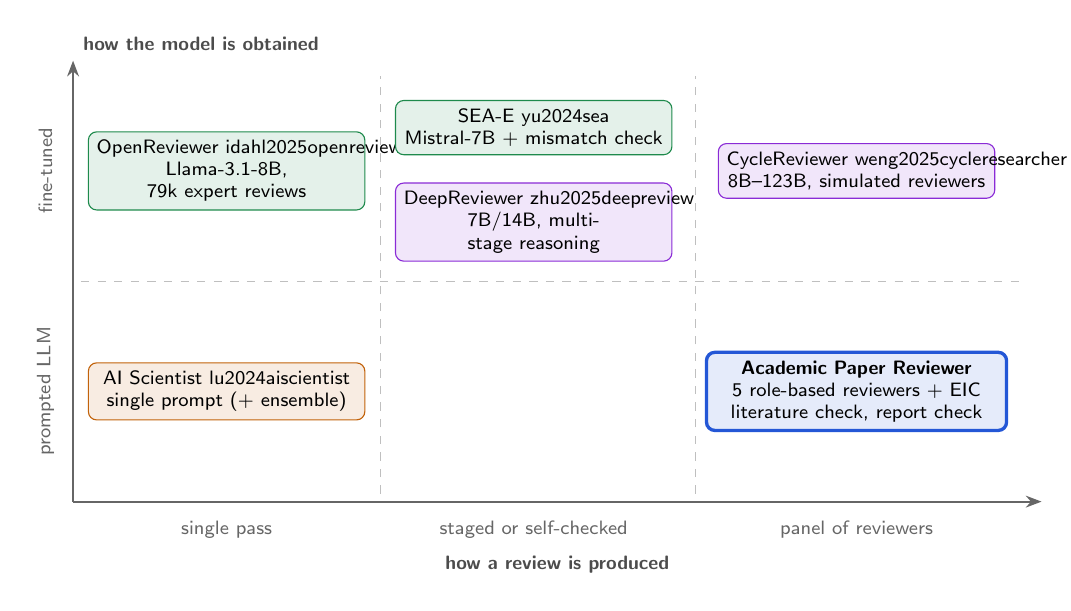
\begin{tikzpicture}[font=\sffamily\small, >={Stealth[length=2mm]},
  sys/.style={draw=#1, fill=#1!12, rounded corners=3pt, align=center, inner sep=3pt, font=\sffamily\scriptsize, text width=33mm, execute at begin node=\hyphenpenalty10000\relax},
  ax/.style={->, thick, draw=black!60}]
\draw[ax] (0,0) -- (12.3,0);
\node[font=\sffamily\scriptsize\bfseries, text=black!70] at (6.15,-0.8) {how a review is produced};
\draw[ax] (0,0) -- (0,5.6) node[above right, font=\sffamily\scriptsize\bfseries, text=black!70] {how the model is obtained};
\foreach \x/\t in {1.95/single pass, 5.85/staged or self-checked, 9.95/panel of reviewers}
  \node[font=\sffamily\scriptsize, text=black!60] at (\x,-0.35) {\t};
\node[font=\sffamily\scriptsize, text=black!60, rotate=90] at (-0.35,1.4) {prompted LLM};
\node[font=\sffamily\scriptsize, text=black!60, rotate=90] at (-0.35,4.2) {fine-tuned};
\draw[dashed, draw=black!25] (0.1,2.8) -- (12.1,2.8);
\draw[dashed, draw=black!25] (3.9,0.1) -- (3.9,5.4);
\draw[dashed, draw=black!25] (7.9,0.1) -- (7.9,5.4);
\node[sys=cG] (ais) at (1.95,1.4) {AI Scientist~\citep{lu2024aiscientist}\\single prompt (+ ensemble)};
\node[sys=cD] (or) at (1.95,4.2) {OpenReviewer~\citep{idahl2025openreviewer}\\Llama-3.1-8B,\\79k expert reviews};
\node[sys=cD] (sea) at (5.85,4.75) {SEA-E~\citep{yu2024sea}\\Mistral-7B + mismatch check};
\node[sys=cP] (dr) at (5.85,3.55) {DeepReviewer~\citep{zhu2025deepreview}\\7B/14B, multi-stage reasoning};
\node[sys=cP] (cr) at (9.95,4.2) {CycleReviewer~\citep{weng2025cycleresearcher}\\8B--123B, simulated reviewers};
\node[sys=cM, very thick, text width=36mm] (us) at (9.95,1.4) {\textbf{Academic Paper Reviewer}\\5 role-based reviewers + EIC\\literature check, report check};
\end{tikzpicture}
\caption{Design space of AI reviewers. Fine-tuned systems learn from public reviews of past
conferences. Our skill prompts a strong general model through a structured panel and needs no
training data. Positions are qualitative.}
\label{fig:design}
\end{figure}

\paragraph{Reported scores of reviewer models.}
Table~\ref{tab:sys} collects published score-agreement numbers. They come from different paper
sets, sizes and targets and are \emph{not} comparable with our 20-paper pilot. Because all the
fine-tuned models were trained on data up to ICLR 2024--2025, ICLR 2026 is unseen by them, which
makes them fair open-weight baselines for our sample (future work).

\begin{table}[t]
\centering\small
\caption{Published rating agreement with the mean human rating (1--10 scale). Values are from
\citet{zhu2025deepreview}, Table~2 (columns ICLR 2024 / ICLR 2025). Last row: our pilot.}
\label{tab:sys}
\begin{tabular}{lccc}
\toprule
System & Spearman & Rating MAE & Decision acc.\\
\midrule
DeepReviewer-14B~\citep{zhu2025deepreview} & 0.356 / 0.405 & 0.91 / 0.92 & 0.64 / 0.69\\
CycleReviewer-70B~\citep{weng2025cycleresearcher} & 0.336 / 0.267 & 1.25 / 1.21 & 0.63 / 0.68\\
CycleReviewer-8B~\citep{weng2025cycleresearcher} & 0.280 / 0.279 & 1.24 / 1.21 & 0.64 / 0.68\\
AI Scientist, DeepSeek-R1~\citep{lu2024aiscientist} & 0.326 / 0.324 & 1.65 / 1.81 & 0.52 / 0.43\\
AI Scientist, Claude 3.5 Sonnet~\citep{lu2024aiscientist} & 0.037 / $-0.022$ & 1.50 / 1.35 & 0.48 / 0.56\\
\midrule
Ours, Sonnet high, panel rating (ICLR 2026, $n=20$) & 0.48 & 0.79$^\dagger$ & --\\
\bottomrule
\multicolumn{4}{l}{\footnotesize $^\dagger$ On the ICLR 2026 0--10 scale (NMAE $0.079\times10$).}
\end{tabular}
\end{table}

Other studies report MAE 0.86 for OpenReviewer-8B and 1.10 for SEA-E under their own
setup~\citep{li2026beyondrating}. NAIPv2~\citep{zhao2025naipv2} could not reproduce these
systems and quotes their published numbers. Re$^2$~\citep{zhang2025re2} evaluates all four
fine-tuned systems on its review and rebuttal data.

\paragraph{Benchmarks.}
\begin{description}
\item[paperreview.ai~\citep{paperreview}.] Score agreement and acceptance AUC on ICLR; our
protocol follows it.
\item[CSPaper~\citep{cspaper}.] A score-prediction leaderboard with NMAE, NME, SRC and average
word count; we adopt its error metrics.
\item[CoCoReviewBench~\citep{deng2026cocoreviewbench}.] This benchmark scores review
\emph{content} rather than scores. It covers 3{,}900 ICLR 2017--2025 and NeurIPS 2021--2024 papers,
with human references filtered for correctness through reviewer--reviewer and reviewer--author
conflicts, using the meta-review as context. An LLM judge scores correctness, thoroughness,
grounding, verifiability and clarity per category, and the benchmark also reports category
completeness. Among its findings: lexical metrics reward overlap rather than correctness, reasoning
models (including DeepReviewer-14B) match or beat humans on grounding and verifiability, and AI
reviews are broad but shallow.
\item[AI-text detection~\citep{yu2025detect}.] About 789k paired human and AI reviews for
\emph{detecting} AI-written reviews. It has a different goal and a restrictive license, so we do
not use it.
\end{description}

\section{Limitations and future work}
\begin{itemize}
\item \textbf{Sample size.} The full evaluation has 86 papers; its Spearman interval is still
$0.27$--$0.64$, and the Gap Scout test and the 2.11 comparison use the 20-paper pilot only.
Haiku and the two GPT-6.1 models were tested on the pilot's 20 papers only.
\item \textbf{No gain over the plain model on agreement with humans.} Section~\ref{sec:control}
finds the same ranking, acceptance AUC, hit rate and precision without the skill. The control was
run once per paper with one prompt, and the planted-defect comparison covers three papers.
\item \textbf{One venue and one year.} Calibration covers ICLR 2026 only. Other venues use
assumed or secondary scales.
\item \textbf{Memorization.} Strong models recognize some papers. We report recognized papers
separately but cannot detect unreported recognition.
\item \textbf{Scores are not the review.} Ranking agreement says nothing about whether the stated
weaknesses are correct, and the overlap study (Section~\ref{sec:overlap}) measures agreement with
humans, not correctness. A content-level evaluation (for example
CoCoReviewBench~\citep{deng2026cocoreviewbench}) is the natural next step, together with
open-weight baselines~\citep{zhu2025deepreview,weng2025cycleresearcher} run on the same ICLR 2026
papers.
\item \textbf{The Gap Scout's items are unchecked.} Its list is longer than a human panel's,
and part of its hit rate is volume; how many of its items are wrong or already answered by the
paper was not measured.
\item \textbf{Compressed ratings.} On the 86 papers, 78\% receive final Overall 3 (ICLR 4);
accepted papers are rated 0.8 points below the humans. Better ranking at the top and bottom of
the pool is the main open problem.
\item \textbf{Human labels are noisy.} On the 86 papers, one human agrees with another at only
Spearman 0.14. Mean human ratings are a weak target, and acceptance is a coarse one.
\end{itemize}

\section*{Reproducibility}
The skill, the scoring script, the evaluation harness, per-paper scores and paper IDs are in the
repository. Manuscripts and review text are not committed. Key commands:
{\small\begin{verbatim}
python3 -m unittest discover -s tests -v
python3 evals/iclr_calibration.py features RESULTS_DIR --out features.jsonl
python3 evals/iclr_calibration.py pilot sample.jsonl features.jsonl
python3 evals/iclr_calibration.py evaluate sample.jsonl features.jsonl \
        --splits splits.json
\end{verbatim}}
Paid runs use the workflow \code{.github/workflows/}\allowbreak\code{iclr-calibration.yml},
configured by \code{evals/iclr\_run.json}.


\begin{thebibliography}{99}\small
\bibitem[Deng et~al.(2026)]{deng2026cocoreviewbench}
H.~Deng, X.~Ke, Y.~Li, et~al.
\newblock CoCoReviewBench: A completeness- and correctness-oriented benchmark for AI reviewers.
\newblock arXiv:2605.07905, 2026.

\bibitem[Idahl and Ahmadi(2025)]{idahl2025openreviewer}
M.~Idahl and Z.~Ahmadi.
\newblock OpenReviewer: A specialized large language model for generating critical scientific
paper reviews.
\newblock In \emph{NAACL 2025 System Demonstrations}. arXiv:2412.11948.

\bibitem[Li et~al.(2026)]{li2026beyondrating}
B.~Li, H.~Ma, Y.~Wang, et~al.
\newblock Beyond rating: A comprehensive evaluation and benchmark for AI reviews.
\newblock arXiv:2604.19502, 2026.

\bibitem[Lu et~al.(2024)]{lu2024aiscientist}
C.~Lu, C.~Lu, R.~T. Lange, et~al.
\newblock The AI Scientist: Towards fully automated open-ended scientific discovery.
\newblock arXiv:2408.06292, 2024.

\bibitem[paperreview.ai(2025)]{paperreview}
paperreview.ai.
\newblock Technical overview.
\newblock \url{https://paperreview.ai/tech-overview}.

\bibitem[CSPaper(2026)]{cspaper}
CSPaper.
\newblock AI review benchmark.
\newblock \url{https://cspaper.org/benchmark}.

\bibitem[Weng et~al.(2025)]{weng2025cycleresearcher}
Y.~Weng, M.~Zhu, G.~Bao, et~al.
\newblock CycleResearcher: Improving automated research via automated review.
\newblock In \emph{ICLR}, 2025. arXiv:2411.00816.

\bibitem[Yu et~al.(2024)]{yu2024sea}
J.~Yu, Z.~Ding, J.~Tan, et~al.
\newblock Automated peer reviewing in paper SEA: Standardization, evaluation, and analysis.
\newblock In \emph{Findings of EMNLP}, 2024. arXiv:2407.12857.

\bibitem[Yu et~al.(2025)]{yu2025detect}
S.~Yu, M.~Luo, A.~Madasu, V.~Lal, and P.~Howard.
\newblock Is your paper being reviewed by an LLM? Benchmarking AI text detection in peer review.
\newblock arXiv:2502.19614, 2025.

\bibitem[Zhang et~al.(2025)]{zhang2025re2}
D.~Zhang, Z.~Bao, S.~Du, et~al.
\newblock Re$^2$: A consistency-ensured dataset for full-stage peer review and multi-turn rebuttal
discussions.
\newblock arXiv:2505.07920, 2025.

\bibitem[Zhao et~al.(2025)]{zhao2025naipv2}
P.~Zhao, J.~Tian, Q.~Xing, et~al.
\newblock NAIPv2: Debiased pairwise learning for efficient paper quality estimation.
\newblock arXiv:2509.25179, 2025.

\bibitem[Zhu et~al.(2025)]{zhu2025deepreview}
M.~Zhu, Y.~Weng, L.~Yang, and Y.~Zhang.
\newblock DeepReview: Improving LLM-based paper review with human-like deep thinking process.
\newblock In \emph{ACL}, 2025. arXiv:2503.08569.
\end{thebibliography}

\appendix
\section{Per-paper pilot scores}
\begin{center}\small
\begin{tabular}{llrrrrrc}
\toprule
& & Human & \multicolumn{2}{c}{Haiku} & \multicolumn{2}{c}{Sonnet high} & \\
\cmidrule(lr){4-5}\cmidrule(lr){6-7}
Paper & Decision & mean & panel & pool & panel & pool & Recognized\\
\midrule
\texttt{AIKURJjxXT} & Withdrawn & 2.50 & 3.2 & 40 & 2.8 & 40 &  \\
\texttt{KtocialdxS} & Reject & 2.67 & 3.4 & 48 & 3.0 & 45 &  \\
\texttt{8xcmfwomnI} & Reject & 3.00 & 3.0 & 40 & 3.0 & 42 &  \\
\texttt{g4HpTtgsn2} & Withdrawn & 3.00 & 3.2 & 46 & 2.6 & 38 &  \\
\texttt{E5mL07Fbq8} & Reject & 3.33 & 3.0 & 38 & 2.6 & 42 &  \\
\texttt{Z6z4AnXGhw} & Reject & 3.50 & 3.4 & 50 & 3.2 & 50 &  \\
\texttt{gUw8n109ki} & Withdrawn & 3.50 & 3.2 & 50 & 2.6 & 40 &  \\
\texttt{0xObmDmsKY} & Reject & 4.00 & 3.2 & 46 & 3.0 & 45 &  \\
\texttt{BxeJLOrKDF} & Withdrawn & 4.00 & 3.2 & 45 & 3.2 & 45 &  \\
\texttt{Jw7khYzYzl} & Reject & 4.00 & 3.6 & 45 & 4.0 & 70 & \checkmark \\
\texttt{9jcB40wjk3} & Accept & 4.40 & 2.8 & 40 & 2.8 & 38 &  \\
\texttt{be4ey66fhk} & Reject & 4.40 & 3.2 & 45 & 3.4 & 52 &  \\
\texttt{9R2iUHhVfr} & Reject & 4.50 & 3.4 & 50 & 3.6 & 65 & \checkmark \\
\texttt{PJdMrK79Mo} & Accept & 4.50 & 3.6 & 48 & 3.4 & 50 &  \\
\texttt{qfW4IrUuig} & Reject & 4.50 & 3.0 & 40 & 2.8 & 40 &  \\
\texttt{Lvkbe0CgmZ} & Reject & 5.00 & 3.4 & 40 & 3.2 & 45 &  \\
\texttt{tlYSbw5GXY} & Accept & 5.20 & 3.2 & 38 & 3.4 & 55 &  \\
\texttt{euMVC1DO4k} & Accept & 6.00 & 3.6 & 50 & 3.8 & 68 & \checkmark \\
\texttt{kwro5432AI} & Desk rej. & 6.00 & 3.2 & 45 & 3.0 & 42 &  \\
\texttt{rubeJmT1XM} & Accept & 6.00 & 3.2 & 40 & 3.0 & 40 &  \\
\bottomrule
\end{tabular}
\end{center}
Human mean is on the ICLR 2026 scale (0--10). ``Panel'' is the reviewers' mean Overall (1--6) and
``pool'' is the EIC pool position (0--100).

\end{document}
